\chapter[DDDC with NMP plant dynamics]{Direct-Data Driven Control in presence of Non-Minimum Phase plant dynamics}

Designing a controller for a \textbf{non-minimum phase system} is challenging since, no matter what is the used approach for designing it, there will be very commonly \underline{unstable zero-pole cancellations}.\\
Moreover, in the framework of Set-Membership DDDC, the plant is unknown and no estimate of the NMP zeros is done. The approach proposed in \citeauthor{cerone2017_NMP} \cite{cerone2017_NMP} deals with a \textbf{two-stage systematic procedure} in order to detect and manage the presence of non-minimum phase dynamics in the plant to be controlled. 

\section{Two stage procedure for DDDC of NMP plant}
Before starting, it is crucial to give the definition of \textbf{prospective plant $G^*$}:
\begin{definition}[\textbf{PROSPECTIVE PLANT}]
    Given a reference model with transfer function $M$ and a designed controller with transfer function $K$, the \textit{prospective plant} $G^*$  is defined as 
    \begin{equation}
        G^*=\frac{M}{K(1-M)}
    \end{equation}
    moreover given the designed controller $K$, the prospective plant $G^*$ is the one giving a closed-loop transfer function that perfectly match the reference model in $M$.
\end{definition}

Using the notion of \textit{prospective plant $G^*$} we have just defined the following procedure allows the user to detect if the designed controller is leading to unstable zero-pole cancellations.

\subsection{Stage \#1: Controller design and detection of unstable zero-pole cancellations}
Given some collected data $\{r,\tilde{y}\}_k$ and a reference model $M(q^{-1})$ a controller $K(q^{-1},\rho)$ is designed following the procedure described in \Cref{chap:DDDC}. At this point, there are two cases:
\begin{enumerate}
    \itemsep-0.3em
    \item \textsf{Stable $K(\rho)$} The controller can be realized, since no unstable cancellations can occur! (The controller is stable).
    \item \textsf{Unstable $K(\rho)$} You have to reject the obtained $K(\rho)$ and adopt one of the following two approaches.
\end{enumerate}

\subsubsection{1st approach: Enforcing stability for $K(\rho)$}
Using the notions presented in \Cref{chap:enforcing}, by adding to the FCPS a proper number of constraints. Such an approach is a conservative one. 
\subsubsection{2nd approach: go to Stage \#2}


\subsection{Second stage: $M$ modification and re-design of $K$}
All the unstable poles of the designed controller $K(\rho)$ close to the NMP zeros must be added in a suitable way to the reference model $M$, if the reference model is designed according to the $\mathcal{H}_\infty$ fictitious control problem, you have to put such poles as NMP zeros of the \textit{fictitious plant} $\tilde{G}$, together with a number of poles equals or greater than the unstable ones.

\begin{figure}[h]
    \centering 
    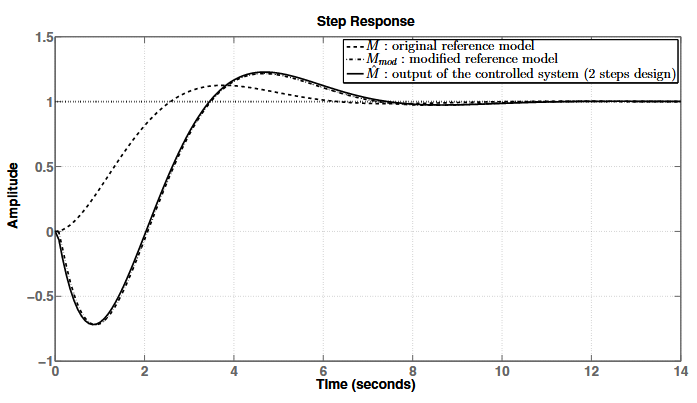
\includegraphics[scale=1]{img/NMP_1.png}
    \caption{Comparison of step responses: designed feedback control system (2 step-procedure) (solid), the original reference model(dashed), modified reference model (dashed-dotted)}
\end{figure}